\documentclass[a4paper, 12pt]{report}

\usepackage[utf8]{inputenc}
\usepackage[T1]{fontenc}
\usepackage[francais]{babel}
\usepackage{graphicx}
\usepackage{amsthm}
\usepackage{amsfonts}
\usepackage{amssymb}
\usepackage{amsmath}
\usepackage{textcomp}
\usepackage{hyperref}
\usepackage{stmaryrd} %llbracket and rrbracket
\usepackage{ dsfont }
\usepackage{mathrsfs}


%Liens hypertexte
\hypersetup{
    colorlinks,
    citecolor=black,
    filecolor=black,
    linkcolor=blue,
    urlcolor=black
}

%Découpe des mots
\hyphenation{}

%Alinéa
%\setlength{\parindent}{2 cm}


\setcounter{tocdepth}{1}
\setcounter{secnumdepth}{1}

%Paramètre de la page
\headheight=0mm
\topmargin=-10mm
\oddsidemargin=-1cm
\evensidemargin=-1cm
\textwidth=18cm
\textheight=25.5cm
\parindent=0mm



%Création du Titre
\title{ \bf Fractales et dimension de Hausdorff}
\author{Mechineau Alexandre}

\makeindex




\begin{document}
	%Creation du paragraphe définition
	\newtheorem{definition}{Définition}
	\newtheorem{prop}{Proposition}
	\newtheorem{theorem}{Théorème}
	\newtheorem*{remark*}{Remarque}
	\newtheorem{lemma}{Lemme}
	
	
	\maketitle
	
	\begin{abstract}
		Je vais définir ce qu'est un ensemble auto-similaire puis chercher à caractériser sa dimension dans l'espace. De plus, je ferais le lien entre fractale et ensemble auto-similaire. Pour terminer, je montrerai définirai quelques fractales.
	\end{abstract}
	
	\tableofcontents
	
	\chapter{\bf Introduction}
		
		Le mot fractale a été introduit par Benoît Mandelbrot, en 1974, pour décrire des objet brisés mais invariants aux changements d'échelle. C'est à dire que lorsque l'on zoome sur une partie d'une fractale on voit le même motif qu'avant.
		
		Cependant, ces objets avaient déjà été remarqués, dés l'antiquité par Apollonius de Perge avec la figure en son nom ``la baderne d'Apollonius''.
		\begin{center}
			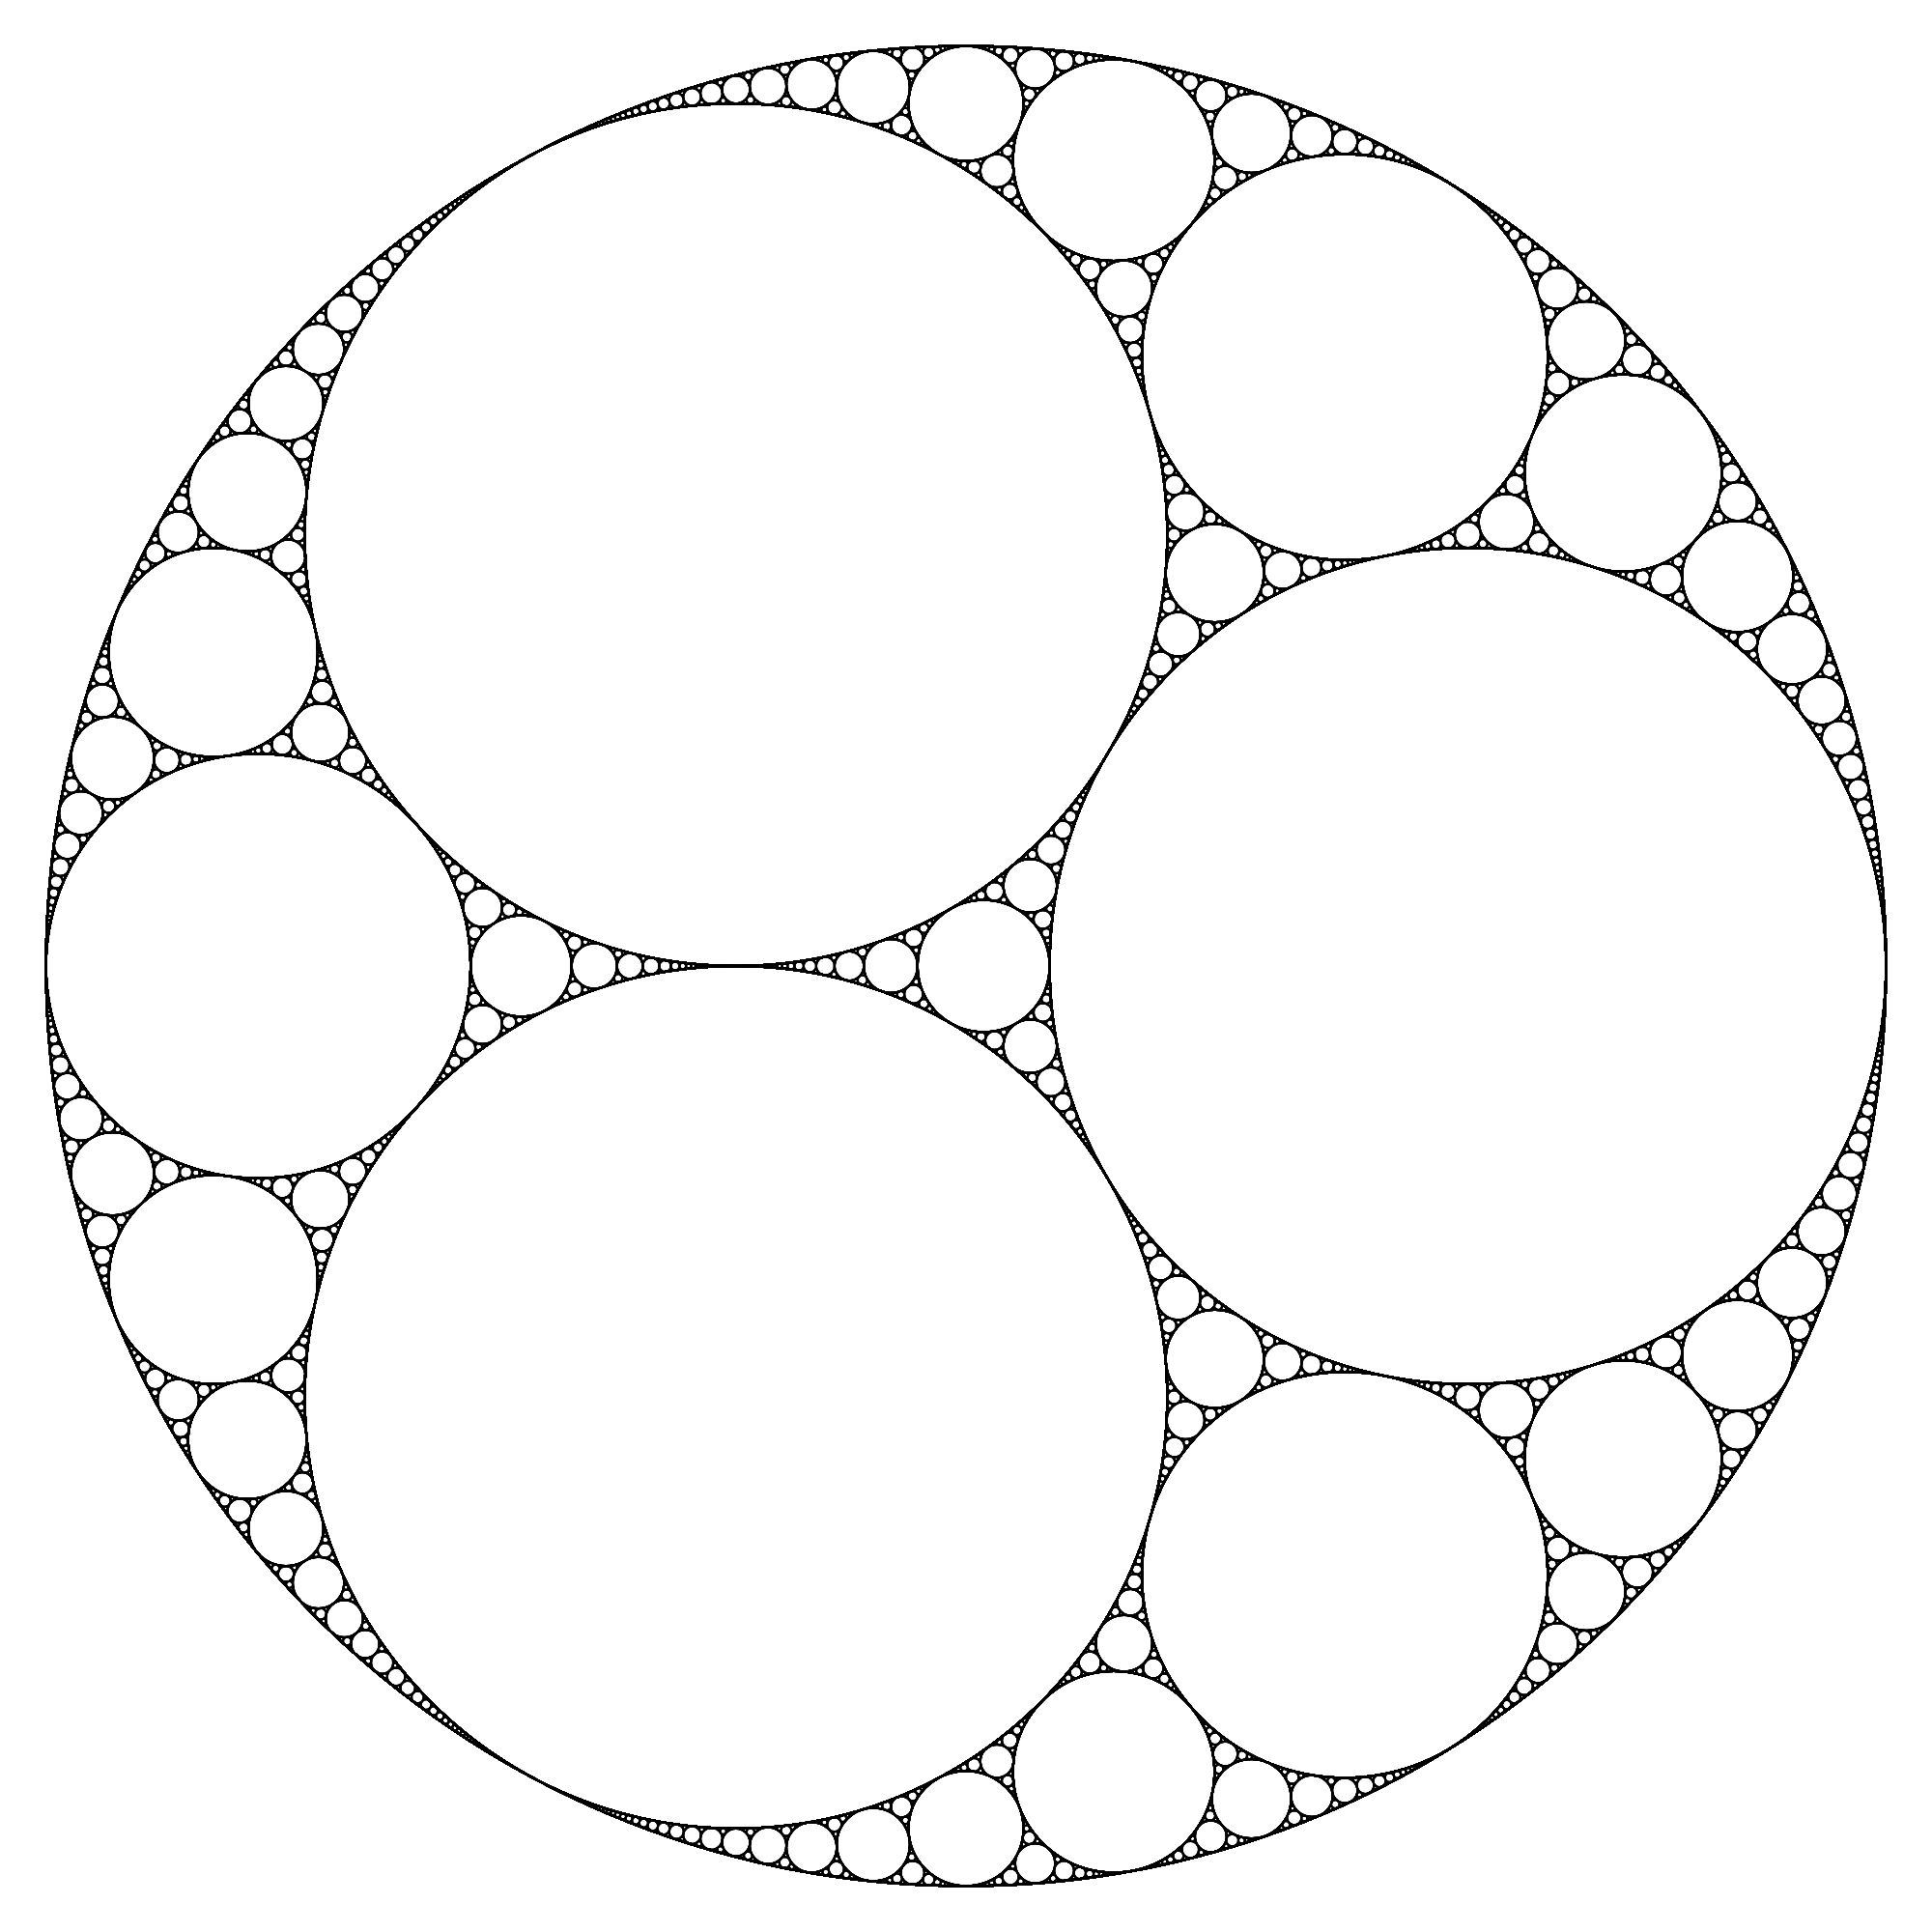
\includegraphics[scale=0.1]{Images/baderne}
		\end{center}
		
		\hspace{.7 cm} Dürer, en 1520, dessine une fractale que l'on nommera ``Pentagone de Dürer''. On l'étudiera sous le nom de \hyperref[Pentakun]{Pentakun}. 
		
		
		\hspace{.7 cm} De plus,  ces figures se retrouvent souvent dans la nature,  c'est le cas du chou Romanesco. On peut aussi citer le cas des poumons, le fait d'avoir une géométrie fractale permet d'avoir une surface importante avec un volume très petit.
		
		\hspace{.7 cm} Il existe trois types de fractale. La première étudie la convergence d'une suite en fonction des points du plan, la seconde, est un système d'itération de fonctions et la dernière utilise le hasard.
		
		\hspace{.7 cm}Nous allons étudier la seconde nommée IFS. Pour cela, nous commencerons par un petit rappel sur les ensembles (compacts,....), puis nous introduirons la notion d'ensemble auto-similaire. Dans un second temps, nous chercherons à caractériser la dimension des ensembles auto-similaires. Enfin, nous découvrirons quelques fractales.	
	
	\chapter{\bf Ensemble auto-similaire et fractale}
		\section{Rappel}
			Dans un premier temps je vais définir ce qu'est un espace métrique. Puis, je rappellerai quelques notions sur les espaces complets et les espaces compacts. Enfin, je rappellerai la notion d'application contractante et énoncerai le Théorème du point fixe de Banach(Picard).
			
			\begin{definition}
				On appelle $(E,d)$ un \textbf{espace métrique} si $E$ est un ensemble et $d$ une distance sur E.
				
				On appelle distance sur un ensemble $E$ une application:
				\begin{equation*}
					d:E^2\longrightarrow \mathds{R}
				\end{equation*}
			Tel que pour tout $x$,$y$,$z$ $\in E$:
				\begin{enumerate}\itemsep2pt
					\item $d(x,y)=d(y,x)$
					\item $d(x,y)=0 \Longrightarrow x=y$
					\item $d(x,z) \leq d(x,y)+d(y,z)$
				\end{enumerate}
			\end{definition}
			
			\begin{definition}
				Un ensemble $X$ d'un espace métrique $(E,d)$ est dit \textbf{complet} si toute suite de Cauchy dans $X$ admettent une limite dans $X$.
				\label{espMetriqueDef}
			\end{definition}
			
			\begin{definition}
				Un ensemble $X$ d'un espace métrique $(E,d)$ est dit \textbf{pré-compact} si il existe $\varepsilon >0$, on peut recouvrir $X$ par un nombre fini de boule ouverte de rayon $\varepsilon$.
			\end{definition}
			
			\begin{definition}
				Soit $(E,d)$ un espace métrique et $X$ un sous-espace de $E$.
				\begin{itemize}
					\item Un ensemble fini $A$ est appelé \textbf{r-recouvrement} de $X$ si et seulement si:
					\begin{equation*}
						\cup_{x\in A} \mathcal{B}_r(x)\supseteq X,\mathcal{B}_r(x)=\{e\in E\mid d(x,e)<r\}
					\end{equation*}
					\item $X$ est dit \textbf{pré-compact} si et seulement si il existe un r-recouvrement de $X$.
				\end{itemize}
			\end{definition}
			
			\begin{definition}
			\label{compactDef}
				Un ensemble $X$ d'un espace métrique $(E,d)$ est dit \textbf{compact} si pour tout r-recouvrement, il existe un sous-ensemble fini d'ouvert tel que leurs unions contiennent X.
			\end{definition}
			
			\begin{prop}
			\label{compactProp}
				Un ensemble $X$ d'un espace métrique $(E,d)$ est \textbf{compact} si et seulement si il est \textbf{complet} et \textbf{pré-compact}.
			\end{prop}
			
			\begin{remark*}
				La définition \ref{compactDef} et la propriété \ref{compactProp} sont équivalentes.
			\end{remark*}

			

			\hspace{.7 cm} On a donc rappelé l'ensemble des notions de topologie nécessaire pour introduire les ensembles auto-similaires. Mais avant, on va rappeler la notion d'application contractante et le Théorème du point fixe de Picard.
			
			\begin{definition}
				Une application $f$ d'un espace métrique $(E,d)$ est dite \textbf{contractante} si:
				\begin{equation}
					\exists k\in\mathds{R}^+, k<1 \mid \forall x,y\in E, d(f(x),f(y))\leqslant k\times d(x,y)
					\label{Pcontractante}
				\end{equation}
			\end{definition}
			
			\begin{remark*}
				Une application est contractante  par rapport à une distance donnée!
			\end{remark*}

			\hspace{.7 cm}Comme nous le verrons plus tard, cette propriété de contraction est la clé pour pouvoir définir ce que sont les fractales définies par IFS et avoir un ensemble limite. On va d'abord montrer qu'une application contractante admet un point fixe.
			
			\begin{theorem}[\textbf{Théorème du points fixe de Banach(Picard)}]
				\label{ThmPtFixe}
				Soit $(E,d)$, un espace métrique complet et $f$ une application k-contractante de $E$ dans $E$. Alors, il existe un unique point fixe $x^*$ de $f$:
				\begin{equation*}
					x^*\in E\mid x^*=f(x^*)
				\end{equation*}
				De plus, pour toute suite d'éléments $(x_n)_{n\in\mathds{N}}$ de $E$ vérifiant la récurrence :
				\begin{equation*}
					x_{n+1}=f(x_n)
				\end{equation*}
				On a,
				\begin{equation}
					d(x_n,x^*)\leq \frac{k^n}{1-k} d(x_0,x_1)
				\end{equation}
				Donc, la suite $(x_n)$ converge vers $x^*$.
				On note aussi, $\forall a\in E,(f^n(a))_{n\geq 0}\longrightarrow x^*$ si $x^*$est un point fixe.
			\end{theorem}

			\begin{proof}
				Soit $(X,d)$ un espace complet.\\
				Soit $f$ une application k-contractante de $E$ dans $E$.\\
				On pose $m,n\in\mathds{N}\mid m>n,a\in E$\\
				\begin{align*}
					d(f^n(a),f^m(a))&\leq d(f^n(a),f^{n+1}(a))+\ldots+d(f^{m-1}(a),f^m(a))  \tag{Inégalité triangulaire}\\
									&\leq (k^n+\ldots+k^{m-1})d(a,f(a)) \tag*{\eqref{Pcontractante}}\\
									&\leq \frac{k^n}{1-k}d(a,f(a))
				\end{align*}
				La série $(f^n(a))_{n\geq 0}$ est donc de Cauchy. Or, E est complet, $(f^n(a))_{n\geq 0}$ admet donc une limite dans $E$ (Définition \ref{espMetriqueDef}). On note cette limite $x^*$.
				On a alors $x^*=f(x^*)$\\
				\textbf{Unicité du point fixe :}
				\begin{align*}
					f(x)=x \textrm{ et } f(y)=y\\
					&d(x,y) = d(f(x),f(y)) \leq k\times d(x,y)\\
					&d(x,y) \leq k\times d(x,y)
					&\Rightarrow d(x,y)=0\Rightarrow x=y \tag{Unicité}
				\end{align*}
			\end{proof}
			\hspace{.7 cm} Le théorème du point fixe de Picard est défini pour une application contractante définie sur un ensemble complet.
\newpage
		\section{Ensemble auto-similaire}
			Les ensembles auto-similaires sont définis à partir d'une union d'ensemble compact, on cherche, alors, un théorème similaire au théorème du point fixe de Picard mais s'appliquant sur une union d'espace compact.
			\begin{theorem}[Théorème de Hutchinson: Unicité et existence des ensembles auto-similaires]
			\label{thmPrincipale}
				Soit $(E,d)$ un espace complet.\\
				$\forall i \in \llbracket 1,N \rrbracket, f_i:E \longrightarrow E$ est une application contractante, par rapport à la distance $d$.\\
				Il existe, alors un compact $K\subset E$, tel que:
				\begin{equation*}
					K=\cup^N_{i=1}f_i(K)
				\end{equation*}
				$K$ est appelé un \textbf{ensemble auto-similaire} défini par :
				\begin{equation*}
					\{f_1,\ldots\,f_N\}
				\end{equation*}
			\end{theorem}
			\begin{remark*}
			\hyperref[ThmPtFixe]{Le Théorème du point fixe de Banach} est un cas particulier de ce théorème avec $N=1$.
			\end{remark*}
		
			Pour simplifier, on pose :
			\begin{equation*}
				F(A)=\cup^N_{i=1}f_i(A)
			\end{equation*}
			\hspace{.7 cm} Avant de faire la preuve de ce théorème clé, on introduit quelques notions qui nous faciliterons la tache. Le théorème du point fixe de Picard travaille avec un élément de $(E,d)$, on peut alors utiliser la distance $d$ sur cet élément. Cependant, le théorème \ref{thmPrincipale} utilise des compacts, on va donc chercher à définir une distance pour les compacts.
			
			On introduit, donc, l'ensemble suivant pour tout $(E,d)$ espace complet:
			\begin{equation*}
				\mathcal{C}(E) : \{A|A\subseteq E, A\textrm{ est un compacte non vide de }E\}
			\end{equation*}
			
			\hspace{.7 cm}On va maintenant définir une distance $\delta$ sur $\mathcal{C}(E)$ nommée \textit{distance de Hausdorff} sur $\mathcal{C}(E)$.
			\begin{prop}
				\label{mesHauss}
				Pour $A,B\in\mathcal{C}(E),$ et $(E,d)$ un espace métrique\\
				On définit $\delta(A,B)=\inf\{r>0\mid U_r(A)\supseteq B, U_r(B)\supseteq A\}$\\
				On pose, pour $r>0$ fixé, $U_r(A)=\{x\in E\mid d(x,y)\leq r,y\in A\}$\\
				$\delta$ est alors une distance sur $\mathcal{C}(E)$.\\
				De plus, si $(E,d)$ est complet alors $(\mathcal{C}(E),\delta)$ est complet. (ADMIS)
			\end{prop}
			\begin{remark*}
				La distance $\delta$ dépend de la distance $d$ de l'ensemble $E$ comme nous pouvons le voir dans la définition. 
			\end{remark*}


			
			
			\begin{theorem}
			\label{ThmConverge}
				Soit $(E,d)$ un espace métrique complet.\\
				Soit 
				\begin{align*}
					F:&\mathcal{C}(E)\longrightarrow \mathcal{C}(E)\\
					&A\longmapsto F(A)=\cup^N_{i=1}f_i(A)
				\end{align*}
				et $f_i:X \longrightarrow X, i\in\llbracket 1,N\rrbracket$\\
				Alors $F$ admet un unique point fixe K. De plus, $\forall A\in\mathcal{C}(E), F^n(A)\longrightarrow K$ quand ${n\to\infty}$ par rapport à la distance de Hausdorff.
			\end{theorem}

			\begin{lemma}
				\label{lemme118}
				$\forall A_1,A_2,B_1,B_2\in\mathcal{C}(E),$ on a :
				\begin{equation}
					\label{HaussMajUnion}
					\delta(A_1\cup A_2 , B_1\cup B_2)\leq \max(\delta(A_1,B_1), \delta(A_2,B_2))
				\end{equation}
			\end{lemma}
		
			\begin{proof}
				Si r>$\max(\delta(A_1,B_1), \delta(A_2,B_2))$, alors $U_r(A_1)\supseteq B_1$ et $U_r(A_2)\supseteq B_2$. Par conséquent, $U_r(A_1\cup A_2)\supseteq B_1\cup B_2$.\\
				De même, $U_r(B_1)\supseteq A_1$ et $U_r(B_2)\supseteq A_2\Longrightarrow U_r(B_1\cup B_2)\supseteq A_1\cup A_2$.\\
				On a donc $r\geq \max(\delta(A_1,B_1), \delta(A_2,B_2)) $ (\ref{HaussMajUnion})
			\end{proof}

			\begin{lemma}
			\label{lemme119}
				Si $f$ est une application $k$-contractante défini de $\mathcal{C}(E)$ dans $\mathcal{C}(E)$, alors :
				\begin{equation}
					\delta(f(A),f(B))\leq k\times \delta(A,B),\forall A,B\in\mathcal{C}(E)
				\end{equation}
			\end{lemma}
			
			\begin{proof}
				On sait qu'il existe $s\geq\delta(A,B)$ tel que:
				\begin{equation*}
					U_s(A)\supseteq B \textrm{ et } U_s(B)\supseteq A,  U_{sk}(f(A))\supseteq f(U_s(A))\supseteq f(B)					
				\end{equation*}
				\begin{equation*}
					U_s(B)\supseteq A \textrm{ et } U_s(A)\supseteq B,  U_{sk}(f(B))\supseteq f(U_s(B))\supseteq f(A)
				\end{equation*}
				On a donc montré que $\delta(f(A),f(B))\leq k*s\leq k*\delta(A,B)$

			\end{proof}

			\begin{proof}[Preuve du théorème]
				On applique le Lemme \ref{lemme118}, on obtient alors:
				\begin{align*}
					\delta(F(A),F(B))	&=\delta(\bigcup_{i=1}^N f_i(A),\bigcup_{i=1}^N f_i(B))\\
										&\leq\max_{1\leq i\leq N}\{\delta(f_i(A),f_i(B))\}
				\end{align*}
				D'après le lemme \ref{lemme119} on a:
				\begin{align*}
					\delta(f_i(A),f_i(B))\leq r_i\times\delta(A,B)
				\end{align*}
				On a alors,
				\begin{align*}
					\delta(F(A),F(B))	&\leq\max_{1\leq i\leq N}\{r_i\times\delta(A,B)\}\\
										&\leq \left\lgroup\max_{1\leq i\leq N}\{r_i\}\right\rgroup\times\delta(A,B)
				\end{align*}
				$F$ est donc une application contractante par rapport à la distance de Hausdorff. D'après la proposition \ref{mesHauss}, on sait que $\mathcal{C}(E)$ est complet donc d'après \hyperref[ThmPtFixe]{Le Théorème du point fixe}, $F$ admet un point fixe.
			\end{proof}
\newpage
		\section{Ensemble auto-similaire et fractale}
		\label{FracEns}
			Un ensemble auto-similaire est la traduction du mot anglais ``self-similarity''. Ce mot décrit le fait qu'un objet présente des similarités peu importe l'échelle à laquelle il est regardé. On va étudier les fractales définies par un système de fonctions contractantes, on sera donc dans le cas des ensembles auto-similaires. On choisit $E=\mathds{R}^2$ et on lui associe la distance usuelle. L'espace métrique défini est complet. On pourra donc utiliser l'ensemble des théorèmes et propositions précédentes. Les fonctions qui définirons notre fractale seront des similitudes contractantes. Nous munirons notre fractale d'un sous-compact de $E=\mathds{R}^2$ qui sera le plus adapté à la fractale même si comme nous pourrons le voir cela n'a pas d'importance sur le papier. 
			\begin{definition}
			\label{simiDef}
				Une \textbf{similitude} est une application de $E$ dans $E$ qui multiplie les distances par un rapport $k$ constant.
			\end{definition}
			\begin{remark*}
				On peut représenter une similitude du plan comme la composée d'une homothétie, d'une rotation(ou symétrie) et d'une translation.
			\end{remark*}
			\begin{prop}
				Soit S une similitude, soit $k$ son rapport,$\theta$ son angle de rotation et $T$ un vecteur de translation. On peut écrire S sous la forme suivante:
				\begin{align*}
					S(X)=k\times M(\theta)\times X+T
				\end{align*}
				On pose M étant une rotation directe ou indirecte:
				\begin{align*}
					M(\theta)\in\Bigg\{
					\begin{pmatrix}
						\cos(\theta) & -\sin(\theta) \\
						\sin(\theta) & cos(\theta) 
					\end{pmatrix}
					,
					\begin{pmatrix}
						\cos(\theta) & \sin(\theta) \\
						\sin(\theta) & -cos(\theta) 
					\end{pmatrix}
					\Bigg\}
				\end{align*}
			\end{prop}
			\begin{prop}
				
				Si $S$ est une similitude de rapport $k<1$, alors elle est contractante.
			\end{prop}
			\begin{proof}
				Une similitude de rapport $k$ multiplie les distances par $k$(Définition \ref{simiDef}). Donc, si $k<1$, c'est une application contractante.
			\end{proof}



			\begin{definition}
				Une fractale $F$ défini par $N$ similitudes $S_i$ contractantes est appelé \textbf{IFS} (Iterated function system).\\
				Soit $C$ un compact, on a alors
				\begin{align*}
					F(C)=\cup^N_{i=1}S_i(C)
				\end{align*}

			\end{definition}
			
			\hspace{.7 cm}On remarque qu'une fractale défini par IFS est un ensemble auto-similaire. On sait alors grâce au théorème \ref{thmPrincipale} qu'il existe un unique points fixe(Compact). De plus, on sait grâce au théorème \ref{ThmConverge} que pour tout compact de $E$ le système converge vers un compact $K$ unique. On sait alors que, pour un compact $C$ donné, $F^n(C)$ tend vers $K$, ($F^n$ représente la composée n-ème de F). En calculant quelques itérations, nous pouvons alors obtenir un résultat ressemblant visuellement à $K$.

	\chapter{\bf Dimension des ensembles auto-similaires, Dimension de Hausdorff}
		On sait exprimer la dimension des objets géométriques classiques comme le point,la droite, le plan,... . Pour définir cette dimension, on compte le nombre de variables nécessaires à désigner un de ses points. On a donc $\dim(point)=0$, $\dim(droite)=1$, $\dim(plan)=2$, $\dim(cube)=3$,... On obtient toujours une dimension entière.\\
		Cependant, pour les fractales on ne peut pas définir une dimension entière. On va donc chercher à définir une dimension pour les fractales.
			
			\begin{definition}
				Soit $(X,d)$ un espace métrique. Pour tout ensemble $A$ borné, on définit:
				\begin{align*}
					\mathscr{H}^s_\delta(A)=\inf\{\sum_{i\leq1}diam(E_i)^s:A\subset\cup_{i\leq1}E_i,diam(E_i)\leq\delta\}\\
					diam(E_i)=\sup_{x,y\in E_i}d(x,y)
					\end{align*}
				On définit aussi:
				\begin{equation*}
					\mathscr{H}^s(A)=\lim_{\delta\rightarrow0}\mathscr{H}^s_\delta(A)
				\end{equation*}
			\end{definition}
			\hspace{0.7 cm} Cette définition montre le fait que l'on essaye de recouvrir de la manière la plus efficace possible l'ensemble $A$.
			

			
			
			\begin{lemma}
			\label{lemme152}
				Soit $(E,d)$ un espace complet. Pour $0\leq s\leq t$
				\begin{align*}
					\mathscr{H}^t_\delta(A)\leq\delta^{t-s}\mathscr{H}^s_\delta(A),\forall A\subseteq E \textrm{ bornée}
				\end{align*}
			\end{lemma}
			\begin{proof}
				Si $A\subseteq \cup_{i\geq 1} A_i$ et $diam(A_i)\leq\delta$ pour tout i, on a alors:
				\begin{align*}
					\sum_{i\geq1}diam(A_i)^t\leqslant\sum_{i\geq1}diam(A_i)^{t-s}diam(A_i)^s\leqslant\delta^{t-s}\sum_{i\geq1}diam(A_i)^s
				\end{align*}
			\end{proof}
\newpage
			On peut donc, grâce au lemme précédent, montré cette proposition:
			\begin{prop}
				Pour tout $A\subseteq E$,
				\begin{equation}
					\label{sHaus}
					\sup\{s:\mathscr{H}^s(A)=\infty\}=\inf\{s:\mathscr{H}^s(A)=0\}
				\end{equation}
			\end{prop}
			\begin{proof}
				D'après le lemme \ref{lemme152}, si $s<t$, on a que $\mathscr{H}^s(A)<\infty$ implique $\mathscr{H}^t(A)=0$. De  même, on a $\mathscr{H}^t(A)>0$ implique $\mathscr{H}^s(A)=\infty$. On remarque donc l'implication \ref{sHaus}
			\end{proof}
			
			
			\begin{definition}[Dimension de Hausdorff]
				La valeur $s$ donnée par l'équation \ref{sHaus} est appelé dimension de Hausdorff de $A$. On la note $dim_H A$.
			\end{definition}
			\begin{remark*}
				Il faut remarquer que comme pour la distance de Hausdorff, la dimension de Hausdorff est basée sur la distance $d$. Elle est donc définie pour une distance donnée.
			\end{remark*}
			
			On a définit la dimension de Hausdorff pour des ensembles bornés quelconques. On peut remarquer que la définition de cette dimension, ne nous permet pas de la calculer de manière explicite. Ce que l'on souhaite,ici, c'est pouvoir la calculer pour les fractales que l'on verra. On sait qu'une fractale IFS est un ensemble auto-similaire. On va donc chercher à définir cette dimension dans le cas des ensembles auto-similaires.
			Ce qui définit un ensemble auto-similaire, ce sont ces applications contractantes caractérisées par leurs rapports. On va, donc ,tenter d'exprimé la dimension de Hausdorff en fonction de ces rapports.
			\newline \hspace{0.7 cm} On va dans un premier temps travailler sur une liste de rapports contractants.
			
			\begin{theorem}
				Soit $N$ rapport contractant $r_i$, on a $r_i<1$. $(r_1,\cdots,r_N)$ est une liste de rapports contractants. Il existe $s\geq0$ tel que:
				
				\begin{equation}
					\sum_{i=1}^N r_i^s =1
				\end{equation}
				$s$ est égale à $0$ si et seulement si $N=1$.
			\end{theorem}
			\begin{proof}
				Si $N=1$, $s=0$ est la seule solution.\\
				Si $N>1$, soit $f$ une fonction définie sur$[0,\infty)$ par:
				\begin{equation}
				\label{sumRatio}
					f(t)=\sum_{i=1}^N r_i^t
				\end{equation}
				On a $f(0)=n$ et $\lim_{t\rightarrow\infty}f(t)=0<1$. $f$ est une somme de fonctions continues, donc est continue. $f$ admet comme dérivée:
				\begin{equation*}
					\sum_{i=1}^N r_i^t\ln r_i<0
				\end{equation*}
				$f$ est donc décroissante. $1$ est compris entre $0$ et $n$.
				D'après le théorème des valeurs intermédiaire, il existe une solution positive à l'équation \ref{sumRatio}.
			\end{proof}
			
			\begin{definition}
				Soit N similitudes $S_i$. Soit $(r_1,\cdots,r_N)$ une liste de rapports contractants. On associe, à chaque similitude $S_i$, le rapport $r_i$. On dit que $(f_1,\cdots,f_N)$ est une réalisation de $(r_1,\cdots,r_N)$.
			\end{definition}

			\begin{definition}
				$s$ est appelé dimension de similitude associé à $(r_1,\cdots,r_N)$.
			\end{definition}
			
			Cependant, on pourrait se dire que l'on a la dimension de notre fractale mais ce n'est pas le cas on a juste:
			\begin{remark*}
				Soit K une fractale et soit $(r_1,\cdots,r_N)$ la liste de rapport contractant associée à $K$ de dimension de similitude $s$. On a alors:
				\begin{equation*}
					\dim(K)\leq s
				\end{equation*}
			\end{remark*}
			
			On a besoin d'ajouter une condition plus forte, qui nous permettrais de dire, $s$ est la dimension de la fractale. Cette condition est appelée ``Condition de Moran''.
			\begin{definition}[Condition de Moran]
				Il existe un ouvert $\mathscr{O}$ tel que:
				\begin{equation}
					\mathscr{O}\supset f_i(\mathscr{O})\forall i \textrm{ et } f_i(\mathscr{O})\cap f_j(\mathscr{O})=\emptyset \forall i\neq j
				\end{equation}
			\end{definition}
			Cette condition traduit le fait que l'ensemble des applications définissant l'ensemble auto-similaire sont différente les unes des autres.
			On peut alors, avec cette condition, énoncé le théorème suivant:
			\begin{theorem}
				\label{thmDim}
				Si $(S_1,\cdots,S_n)$ est une réalisation de $(r_1,\cdots,r_n)$ définis sur l'espace métrique $\mathds{R}^d$ et si la condition de Moran est respectée, on a alors:
				\begin{equation*}
					\dim(K)=s
				\end{equation*}
			\end{theorem}
			\hspace{0.7 cm} Grâce à ce théorème, nous sommes en mesure de calculer la dimension de Hausdorff d'un ensemble auto-similaire et de ce fait, celle d'une fractale IFS. Nous mettrons en application ce théorème pour le calcul de la dimension de Hausdorff des fractales lorsque nous les présenterons.
			

			
	
	\chapter{IFS et informatique}
			
			Comme on l'a vu dans la partie \hyperref[FracEns]{Ensemble auto-similaire et fractale}, on sait que l'on peut décrire une fractale IFS par un ensemble de similitude et un compact. 
			Le choix du compact à seulement de l'importance pour avoir un résultat "correct" le plus rapidement. Pour calculer le premier pas de la fractale on applique chaque similitude sur l'ensemble de départ. On obtient, alors, une liste d'ensembles. Pour la deuxième étape, on utilise la liste d'ensemble précédemment obtenue sur laquelle on applique chaque similitude.
			
			
			\vspace{.2 cm}\hspace{.7 cm}
			On utilise comme compact de base un segment, il nous permet de décrire chaque formes nécessaires aux fractales IFS que l'on représentera. On a alors à chaque étape une liste de segments définis par deux points. Cette liste a une taille qui suit une croissance exponentielle. Mais à chaque itération on se rapproche du point fixe. En pratique, à partir de cinq itérations le résultat est correct à l'échelle normale.
			
			\vspace{.2 cm}\hspace{.7 cm}
			D'un point de vue algorithmique, j'ai créé un objet application qui me permet de représenter l'ensemble des applications nécessaires de $\mathds{R}^2$. Puis j'ai créé des objets représentant des applications plus spécifiques, mais dépendants de Application, comme Rotation, Homothétie, ...
			
			\vspace{.2 cm}\hspace{.7 cm}
			J'ai aussi créé un objet Forme décrivant par un ensemble de points un polygone de $\mathds{R}^2$. Cette objet forme représente un compact, c'est en effet l'union de plusieurs segments qui sont compact.
			
			\vspace{.2 cm}\hspace{.7 cm}
			J'ai écrit un dernier objet Fractale me permettant de définir une fractale IFS comme un ensemble d'Application et un ensemble de Forme.
			
			\vspace{.2 cm}\hspace{.7 cm}
			L'objet Application permet d'appliquer l'application définie sur un ensemble de forme. Ce qui revient à calculer l'image de chaque extrémité des segments définissant l'objet Forme.
	
			\vspace{.2 cm}\hspace{.7 cm}
			En appliquant l'ensemble des Application $n$ fois sur la Forme initiale on obtient la n-ème étape de la construction de la fractale. Il ne reste plus qu'à afficher chaque étape à l'écran.
	
			\begin{remark*}
				L'image d'un segment par une similitude est un segment. En effet, effectuer une rotation, translation ou une homothétie sur un segment donne un segment. Une similitude étant la composée de ces différentes applications, elle donne donc un segment.
			\end{remark*}

	
	\chapter{\bf Exemple de fractales}
		On va, donc dans ce chapitre, découvrir plusieurs fractales. On précisera le compact ``optimum'' et l'ensemble des applications pour chaque fractale. Ensuite, on calculera la dimension de Hausdorff de chaque ensemble.\\
		On va commencer par introduire plusieurs notations qui nous serons utiles par la suite.\\
			Les sources du programme utilisé sont disponible à l'adresse https://github.com/Alexsaphir/CantorFractal
		\section{Notation}
			On sait qu'il existe deux types de similitudes, on va donc les définir. On exprimera, aussi, la similitude représentant une homothétie.
			\vspace{.3cm}
			On note $SD$ les similitudes directes du plan.\newline
			On note $SI$ les similitudes indirectes du plan.\newline
			$M_d(\theta)$ est la matrice de rotation directe du plan d'angle $\theta$.\newline
			$M_i(\theta)$ est la matrice de rotation indirecte du plan d'angle $\theta$.\newline
			$H$ est une homothétie de rapport $k$.
			$x$ est un élément d'un compact de $\mathds{R}$ ou du plan.\newline
			$k$ est le rapport d'une similitude.\newline
			$\theta$ est l'angle d'une similitude.\newline
			$T$ est un vecteur représentant une translation.\newline
			\begin{align*}
				M_D(\theta)&=\left(	\begin{array}{ccc}
								\cos(\theta) &  -\sin(\theta) \\
								\sin(\theta) &  \cos(\theta)  \\
									\end{array} \right)\\
				M_I(\theta)&=\left(	\begin{array}{ccc}
								\cos(\theta) &  \sin(\theta) \\
								\sin(\theta) &  -\cos(\theta)  \\
									\end{array} \right)\\
				SD(x)&=k\times M_D(\theta)\times x + T\\
				SI(x)&=k\times M_I(\theta)\times x + T\\
				H(x)&=k\times M_D(0)\times x +T=k\times x+T
			\end{align*}
			
\newpage
		\section{Cantor}
			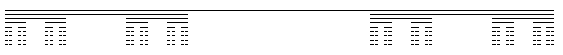
\includegraphics[scale=0.8]{Images/cantor}
			\subsection{Définition}
				Pour l'ensemble de Cantor on part du segment $[0;1]$ que l'on contracte de $1/3$ à droite et gauche.
				On a donc deux homothéties de rapport 1/3 de centre 0 et 1. L'ensemble de départ et d'arrivé pour chaque application est $\mathds{R}.$ 
				\begin{align*}
					&H_1:x\mapsto 1/3\times x\\
					&H_2:x\mapsto 1/3\times x+2/3
				\end{align*}
			\subsection{Dimension}
				Pour calculer la dimension de Hausdorff de l'ensemble de Cantor on utilise le théorème \ref{thmDim}. En effet, comme toute les fractales que nous définirons, l'ensemble de Cantor est constitué de deux similitudes différentes. On a alors,
				\begin{align*}
					\left(\frac{1}{3}\right)^d+\left(\frac{1}{3}\right)^d	&=1\\
											  2\left(\frac{1}{3}\right)^d	&=1\\
											   \left(\frac{1}{3}\right)^d	&=\frac{1}{2}\\
						\exp\left(d\times\ln\left(\frac{1}{3}\right)\right)	&=\frac{1}{2} \tag{Passage à la forme exponentielle}\\
										d\times\ln\left(\frac{1}{3}\right)	&=\ln\left(\frac{1}{2}\right)\\
																		d	&=\frac{\ln\left(\frac{1}{2}\right)}{\ln\left(\frac{1}{3}\right)}\\
																		d	&=\frac{\ln(1)-\ln(2)}{\ln(1)-\ln(2)}\\
																		d	&=\frac{\ln(2)}{\ln(3)} \tag{$\ln(1)$=0}\\
																		d	&\approx 0.6309
				\end{align*}
				On a donc calculer la dimension de Hausdorff de l'ensemble de Cantor.
				
				
				On se base sur ce calcule pour le reste des fractales.
\newpage
		\section{Courbe de Koch}
			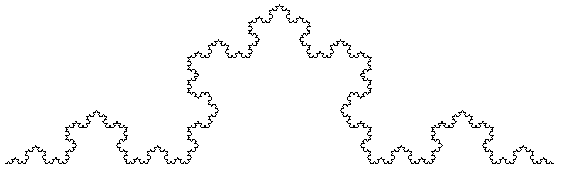
\includegraphics[scale=0.9]{Images/courbe}
			\subsection{Définition}
				Pour la courbe de Koch on part aussi du segment $[0;1]$. On définit quatre similitudes directes du plan.
				\begin{align*}
					&SD_1:x\mapsto 1/3\times x\\
					&SD_2:x\mapsto 1/3\times M_d(\pi/3)\times x+\left(	\begin{array}{ccc}
															1/3\\
															0\\
														\end{array}\right)\\
					&SD_3:x\mapsto 1/3\times M_d(-\pi/3)\times x+\left(	\begin{array}{ccc}
															1/2\\
															\sqrt{3}/6\\
														\end{array}\right)\\
					&SD_4:x\mapsto 1/3\times x+\left(	\begin{array}{ccc}
															2/3\\
															0\\
														\end{array}\right)
				\end{align*}
			\subsection{Dimension}
				La courbe de Koch est constituée de quatre similitudes de rapport $1/3$. On a alors:
				\begin{align*}
					 4\left(\frac{1}{3}\right)^d	&=1\\
												d	&=\frac{\ln(4)}{\ln(3)}\\
												d	&\approx 1.2618
				\end{align*}
\newpage
		\section{Flocon de Koch} 
			\begin{center}
				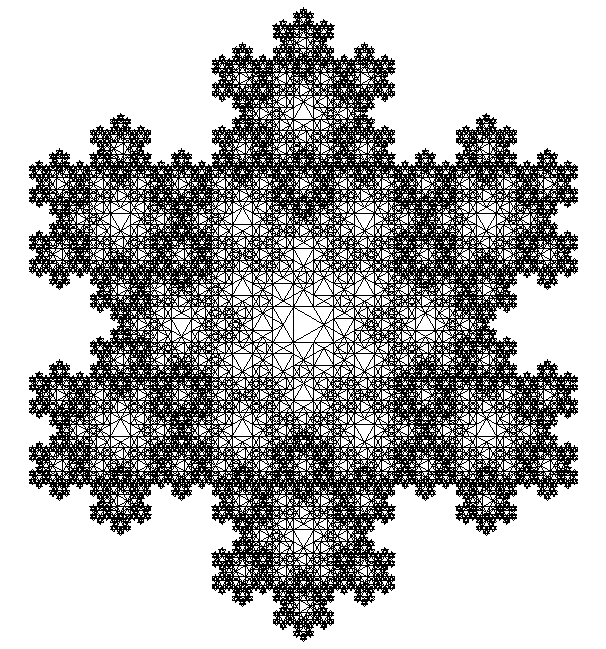
\includegraphics[scale=0.4]{Images/flocon}
			\end{center}
			\subsection{Définition}
				Le flocon de Koch est l'union de trois courbes de Koch. Elle est défini par sept similitudes et la forme de base est un triangle équilatéral de longueur $1$.
				\begin{align*}
					&SD_1:x\mapsto 1/3\times M_d(-2\pi/3)\times x+\left(	\begin{array}{ccc}
															1/6\\
															\sqrt{3}/6\\
														\end{array}\right)\\
					&SD_2:x\mapsto 1/3\times M_d(\pi/3)\times x+\left(	\begin{array}{ccc}
															1/6\\
															\sqrt{3}/6\\
														\end{array}\right)\\
					&SD_3:x\mapsto 1/3\times M_d(0)\times x+\left(	\begin{array}{ccc}
															1/3\\
															\sqrt{3}/3\\
														\end{array}\right)\\
					&SD_4:x\mapsto 1/3\times M_d(-\pi/3)\times x+\left(	\begin{array}{ccc}
															2/3\\
															\sqrt{3}/3\\
														\end{array}\right)\\
					&SD_5:x\mapsto 1/\sqrt{3}\times M_d(\pi/6)\times x+\left(	\begin{array}{ccc}
															1/3\\
															0\\
														\end{array}\right)\\
					&SD_6:x\mapsto 1/3\times M_d(\pi)\times x+\left(	\begin{array}{ccc}
															2/3\\
															0\\
														\end{array}\right)\\
					&SD_7:x\mapsto 1/3\times M_d(0)\times x+\left(	\begin{array}{ccc}
															1/3\\
															0\\
														\end{array}\right)
				\end{align*}
			\subsection{Dimension}
				Le flocon de Koch est constitué de six similitudes de rapport $1/3$ et une similitude de rapport $1/\sqrt{3}$. On a alors:
				\begin{align*}
					 6\left(\frac{1}{3}\right)^d+\left(\frac{1}{\sqrt{3}}\right)^d	&=1\\
																				d	&=2
				\end{align*}
\newpage
		\section{Triangle de Sierpiński}
			\begin{center}
				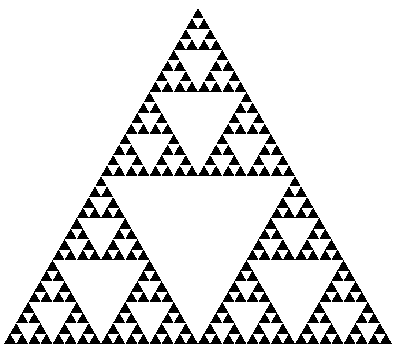
\includegraphics[scale=0.7]{Images/triangle}
			\end{center}
			\subsection{Définition}
				Le triangle de Sierpiński est basé sur un triangle équilatéral de longueur 1. Il est constitué de trois homothéties de centre correspondant aux extrémités du triangle et de rapport $1/2$.
				\begin{align*}
					&H_1:x\mapsto 1/2\times x+\frac{1}{2}\left(	\begin{array}{ccc}
															0\\
															0\\
														\end{array}\right)\\
					&H_2:x\mapsto 1/2\times x+\frac{1}{2}\left(	\begin{array}{ccc}
															1\\
															0\\
														\end{array}\right)\\
					&H_3:x\mapsto 1/2\times x+\frac{1}{2}\left(	\begin{array}{ccc}
															1/2\\
															\sqrt{3/4}\\
														\end{array}\right)
				\end{align*}
			\subsection{Dimension}
				On a pour le triangle de Sierpiński:
				\begin{align*}
					 3\left(\frac{1}{2}\right)^d	&=1\\
												d	&=\frac{\ln(3)}{\ln(2)}\\
												d	&\approx 1.5849
				\end{align*}	
\newpage
		\section{Tapis de Sierpiński}
			\begin{center}
				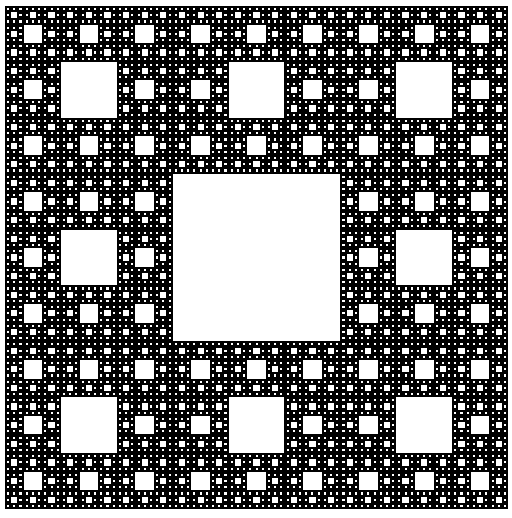
\includegraphics[scale=0.3]{Images/carpet}
			\end{center}
			\subsection{Définition}
				Le tapis de Sierpiński est basé sur un carré, c'est à dire l'union de quatre segments. Il est constitué de 8 homothéties de rapport 1/3.
				\begin{align*}
					&H_1:x\mapsto 1/3\times x+\frac{1}{2}\left(	\begin{array}{ccc}
																0\\
																0\\
															\end{array}\right)\\
					&H_2:x\mapsto 1/3\times x+\frac{1}{2}\left(	\begin{array}{ccc}
																	1\\
																	0\\
																\end{array}\right)\\
					&H_3:x\mapsto 1/3\times x+\frac{1}{2}\left(	\begin{array}{ccc}
																	1\\
																	1\\
																\end{array}\right)\\
					&H_4:x\mapsto 1/3\times x+\frac{1}{2}\left(	\begin{array}{ccc}
																	0\\
																	1\\
																\end{array}\right)\\
					&H_5:x\mapsto 1/3\times x+\frac{1}{2}\left(	\begin{array}{ccc}
																	1/2\\
																	0\\
																\end{array}\right)\\
					&H_6:x\mapsto 1/3\times x+\frac{1}{2}\left(	\begin{array}{ccc}
																	1\\
																	1/2\\
																\end{array}\right)\\
					&H_7:x\mapsto 1/3\times x+\frac{1}{2}\left(	\begin{array}{ccc}
																	1/2\\
																	1\\
																\end{array}\right)\\
					&H_8:x\mapsto 1/3\times x+\frac{1}{2}\left(	\begin{array}{ccc}
																	0\\
																	1/2\\
																\end{array}\right)
				\end{align*}

			\subsection{Dimension}
				En appliquant, la formule une fois encore, on obtient:
				\begin{align*}
					 8\left(\frac{1}{3}\right)^d	&=1\\
												d	&=\frac{\ln(8)}{\ln(3)}\\
												d	&\approx 1.8928
				\end{align*}
\newpage
		\section{Hata's tree-like set}
			\begin{center}
				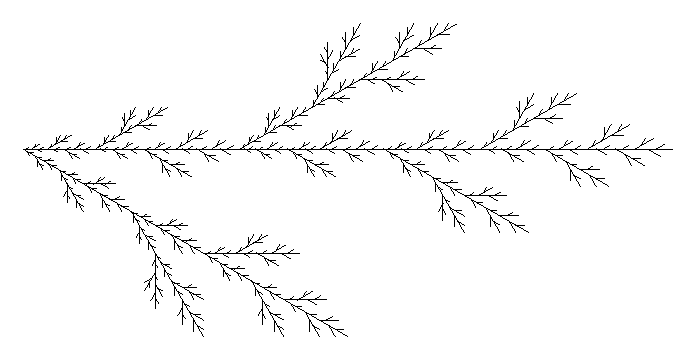
\includegraphics[scale=0.3]{Images/hata1}
				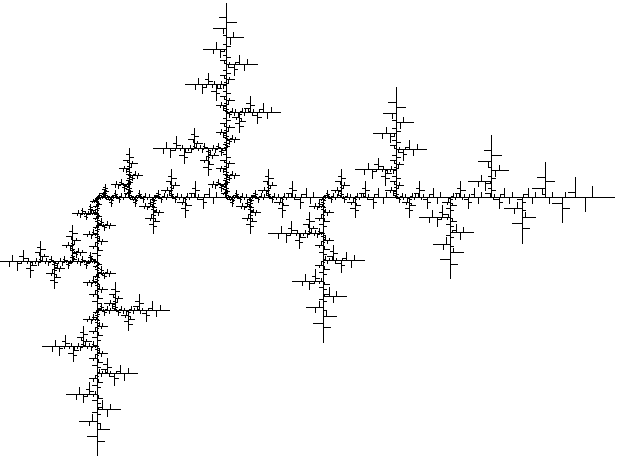
\includegraphics[scale=0.3]{Images/hata2}
			\end{center}
			\subsection{Définition}
				Cette fractale représente de manière simpliste une branche d'arbre. Elle est défini à partir de deux formes le segment classique$[0;1]$ et un second segment ayant pour extrémité l'origine et un point du plan $\beta$ servant de paramètre qui respecte les  conditions suivantes:
				\begin{align*}
					&\left|\beta\right|<1\\
					&\left|\beta-1\right|<1\\
					&\textrm{Im }\beta\neq0
				\end{align*}
				On définit deux similitudes indirectes dépendant de $\beta$:
				\begin{align*}
					SI_1: &x\mapsto \left|\beta\right|\times M_I(\arg(\beta))\times x \\
					SI_2: &x\mapsto(1-\left|\beta\right|^2)\times M_I(0)+ 	\left(\begin{array}{ccc}
																				\left|\beta\right|^2\\
																				0\\
																			\end{array}\right)\\
				\end{align*}
				
				Pour cette fractale, on va l’étudier pour deux paramètres différents:
				\begin{itemize}
					\item $\beta_1=\frac{1}{2}-\frac{1}{2\sqrt{3}}i$ (Image de gauche)
					\item $\beta_2=\frac{1}{2}i$ (Image de droite)
				\end{itemize}
			\subsection{Dimension}
				On doit donc calculer la dimension de deux fractales car le rapport de chaque similitude dépends de $\beta$. J'ai été capable seulement de calculer des valeurs approchées de la dimension de ces deux ensembles.
				Pour $\beta_1$, je trouve une valeur approchée de $1.6355$ et pour $\beta_2$, j'obtiens $1.50713$.
				\begin{align*}
					\left|\beta\right|^r+\left(1-\left|\beta\right|^2\right)^r=1
				\end{align*}


\newpage
		\section{Courbe de Lévy}
			\begin{center}
				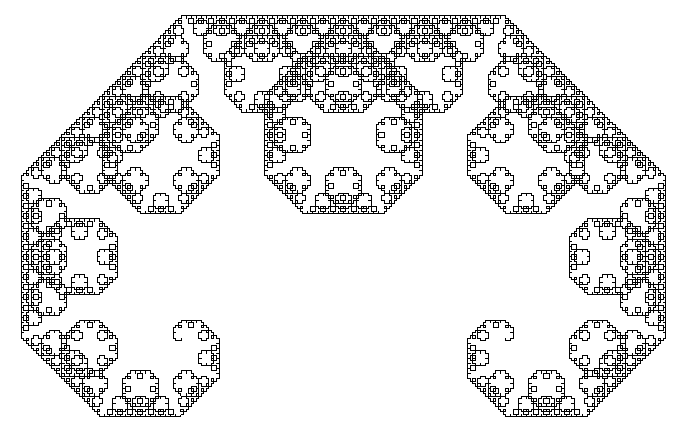
\includegraphics[scale=0.7]{Images/levy}
			\end{center}
			\subsection{Définition}
				La courbe de Lévy est définit à partir d'un segment. Elle est construite par deux similitudes directes de rapport $\frac{\sqrt{2}}{2}$.
			
			\subsection{Dimension}
				\begin{align*}
					 2\left(\frac{1}{\sqrt{2}}\right)^d	&=1\\
					 \left(\frac{1}{\sqrt{2}}\right)^d	&=\frac{1}{2}\\
													d	&=2
				\end{align*}
\newpage
		\section{PentaKun}
		\label{Pentakun}
			\subsection{Définition}
				Le pentakun est basé comme son nom l'indique sur un pentagone. On définit donc cinq points.
				\begin{equation*}
					p_i=\left(\begin{array}{ccc}
							-\sin\left(\frac{2i\pi}{5}\right)\\
							\cos\left(\frac{2i\pi}{5}\right)\\
						\end{array}\right)
						,\forall i\in\textrm{\textlbrackdbl} 1,5\textrm{\textrbrackdbl}
			\end{equation*}
				On définit cinq homothéties qui vont réduire le pentagone dans chaque coin. Le rapport des homothéties est de $\frac{3-\sqrt{5}}{2}$.
				\begin{equation*}
					H_i=\frac{3-\sqrt{5}}{2}\times x+\frac{\sqrt{5}-1}{2}p_i,\forall i\in\textrm{\textlbrackdbl} 1,5\textrm{\textrbrackdbl}
				\end{equation*}
			\subsection{Dimension}
				\begin{align*}
					 5\left(\frac{3-\sqrt{5}}{2}\right)^d	&=1\\
					 \left(\frac{3-\sqrt{5}}{2}\right)^d	&=\frac{1}{5}\\
														d	&=\frac{-\ln(5)}{\ln(3-\sqrt{5})-\ln(2)}\\
														d	&\approx 1.6723
				\end{align*}
				\begin{center}
					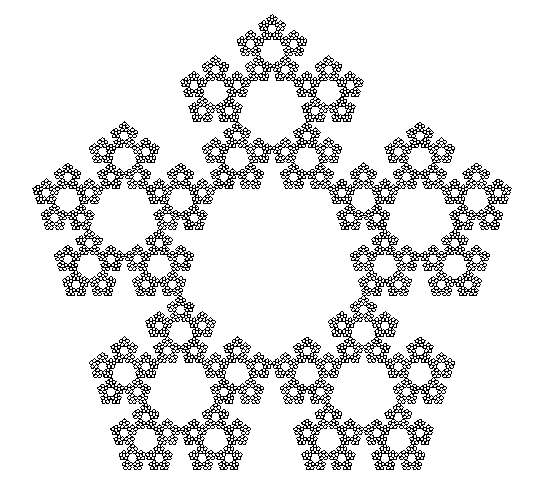
\includegraphics[scale=0.5]{Images/pentakun.png}
				\end{center}
				
	\chapter*{Remerciements}
	\addcontentsline{toc}{chapter}{Remerciements}
	
	Je remercie particulièrement Clément Fromenteau pour ses conseils de qualités tout au long de ce projet.
	\newline
	Je remercie également Théo Voillemin pour les nombreuses corrections orthographiques apportés à ce rapport.
	
	\chapter*{Bibliographie}
	\addcontentsline{toc}{chapter}{Bibliographie}
		\begin{itemize}
			\setlength\itemsep{.5 cm}
			\item KIGAMI, Jun. Hausdorff dimensions of self-similar sets and shortest path metrics. J. Math. Soc. Japan 47 (1995), no. 3, 381--404
			
			\item Jun Kigami . Analysis on Fractals. Cambridge University Press., 2001, ISBN 978-0-521-79321-6
			
			\item J. E. Hutchinson, Fractals and self similarity, Indiana Univ. Math. J. 30 (1981), 713-747.

			\item Classic Iterated Function Systems, \url{http://ecademy.agnesscott.edu/~lriddle/ifs/ifs.htm}, 1999

			\item Wikipedia contributors, 'Totally bounded space', Wikipedia, The Free Encyclopedia, 10 November 2015, 18:06 UTC, \url{https://en.wikipedia.org/w/index.php?title=Totally_bounded_space&oldid=690001055} [accessed 29 April 2016]
			
			\item Shlomo Sternberg, Lecture 10: The Hausdorff metric. Hutchinson's theorem. Fractal images Similarity dimension and Hausdorff dimension., \url{http://www.math.harvard.edu/library/sternberg/slides/1180910.pdf} [accessed 29 april 2016]
		\end{itemize}
\end{document}

\grid
